\documentclass[a4paper, 12pt]{report}
\usepackage[utf8]{inputenc}
\usepackage{graphicx}
\usepackage{xcolor}
\usepackage{appendix}
\usepackage[top=2cm, bottom=2cm, left=2cm, right=2cm]{geometry}
\usepackage[francais]{babel}

\usepackage{fancyhdr}
\usepackage{lastpage}

\addtocontents{toc}{\protect\thispagestyle{fancy}}

\pagestyle{fancy}
\setlength\headheight{12mm}
\fancyhf{}
\lhead{
\includegraphics[height=1cm]{../../public/images/Logo-spf-sm.png}}
\chead{}
\rhead{
\includegraphics[height=8mm]{../../public/images/Logo-entremploi-sm.png}}
\lfoot{\today}
\cfoot{}
\rfoot{page \thepage \ / \pageref{LastPage}}

\title{Entr'Emploi}
\author{MAILLARD Noé MILSONNEAU Jean}

\begin{document}

\begin{titlepage}
	\thispagestyle{empty}
    \centering
    {\bfseries\Large
    		Plateforme web EntrEmploi\\
        \today\\
        \vskip3cm
        
\includegraphics{../../public/images/Logo-entremploi-md.png}
        \vskip15mm
        
\includegraphics{../../public/images/Logo-spf.png}
        \vskip3cm
        Maillard Noé, Milsonneau Jean\\
    }
    \normalsize
\end{titlepage}

\tableofcontents
\newpage
\section*{Introduction}

L'association Entr'Emploi a pour projet depuis le debut de l'année d'avoir a disposition un site internet qui leurs permetterait d'avoir plus de visibilité
dans ce monde numérisé. Malheureusement, l'association n'a, ni les pesonnes compétentes pour réaliser le projet, ni l'argent pour faire appel aux services d'une entreprise.
Nous nous sommes donc proposés d'offir nos capacités pour mettre au jour ce projet, de plus nous y voyions un exellent moyen d'aquérir de l'expérience et de decouvrir de nouvelles technologies.


\chapter{Le projet Entr'Emploi}
\thispagestyle{fancy}
\section{L'action d'Entr'Emploi au secours populaire}
Entr'Emploi propose un accompagnement personnalisé pour les chercheurs d'emploi plus ou moins éloigné du marché du travail depuis cette année dans la région de Brest.\\
Ils les aident à clarifier leur projet, s'orienter vers des formations et à organiser leur recherche d'emploi.\\
Il s'agit de renforcer et de compléter les services proposés par les organismes existants, en apportant aux chômeurs un soutien supplémentaire, structuré et sur le long terme si nécessaire.\\
Ce projet date de 2015 et est mis en place à Brest et également à Quimper, il est très probable que le projet inspire d'autres régions à mettre en place le même programme d'aide.
\section{Notre place dans cette action}
Nous avons répondu à l'appel de l'équipe du secours populaire pour mettre notre passion de l'informatique a leur service.\\
\\
Le but est d'offrir plus de visibilité à l'équipe d'Entr'Emploi tout en leur fournissant un outil de travail pour rendre les chercheurs d'emploi plus visible. Le site doit également permettre de relayer les offres d'emploi que les bénévoles reçoivent.\\
La création du site doit se faire en cohérence et en lien avec le site national du secours populaire tout en offrant sa propre identité au projet Entr'Emploi. Pour nous assurer que nous travaillons dans la bonne direction des réunions régulières sont prévues avec l'équipe de bénévole qui travaillerons avec le site.\\
\\
Notre Rôle est donc d'aider les bénévoles à préparer le plan du site et les fonctionnalités qu'il doit proposer. Nous devons aussi nous montrer réalistes et parfois proposer des compromis pour s'assurer de fournir un site complet et fonctionnel. Les trois premières réunions sont faites pour s'assurer que la bonne direction est donc prise\\

\chapter{Analyse de l’opération}
\thispagestyle{fancy}
\section{Pourquoi une plate-forme web}
\section{Fonctionnalités du site}

\chapter{Calendrier prévisionnel}
\thispagestyle{fancy}
\section{Dates clés}
\section{Réunions}

\chapter{Résultats envisagés}
\thispagestyle{fancy}
\section{Outils de mesure}
\section{Objectif visé}

\newpage
\appendix
\chapter{}
\thispagestyle{fancy}
\section{Charte Graphique}
La charte graphique de notre projet est un élément centrale de notre travail qui évolue avec le reste du projet. On peut tout de même aujourd'hui fixer certaines règles que nous devrons respecter. Nous avons fait le choix de coller au logo actuel du secours populaire.\\
\\
\begin{tabular}{ c  p{10cm}  p{6cm}  }
\raisebox{-\totalheight}{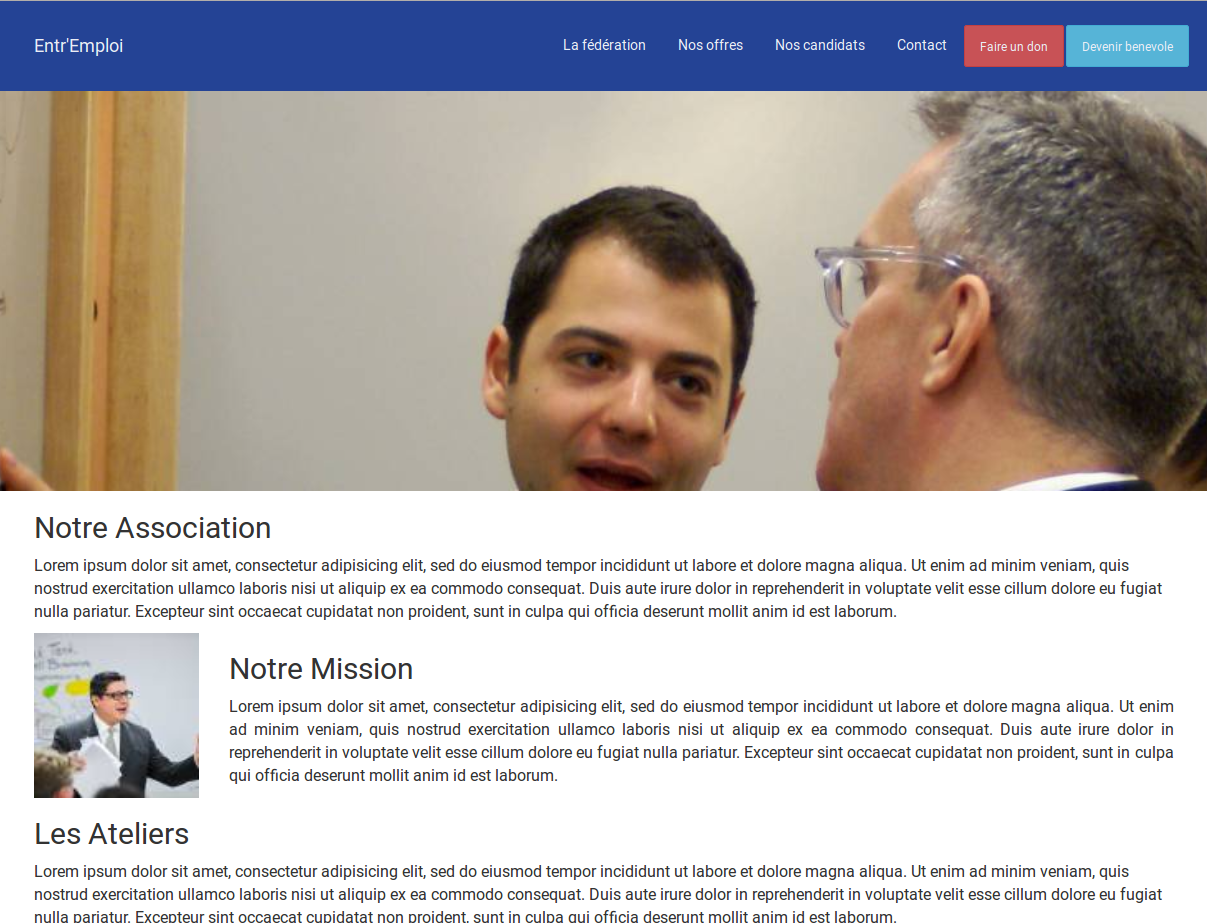
\includegraphics[width=6cm]{maquette1.png}}
&
Notre charte graphique est donc sobre, principalement composé de bleu, blanc et rouge. le bleu étant utilisé pour les menus alors que le rouge trouve sa place pour les boutons et informations importantes. Le visuel ci-contre provient de la première maquette qui va évoluer pour, notamment, se rapprocher plus du visuel du site du secours populaire (Cf A.5).\\
\end{tabular}

\section{Diagramme de Gantt}
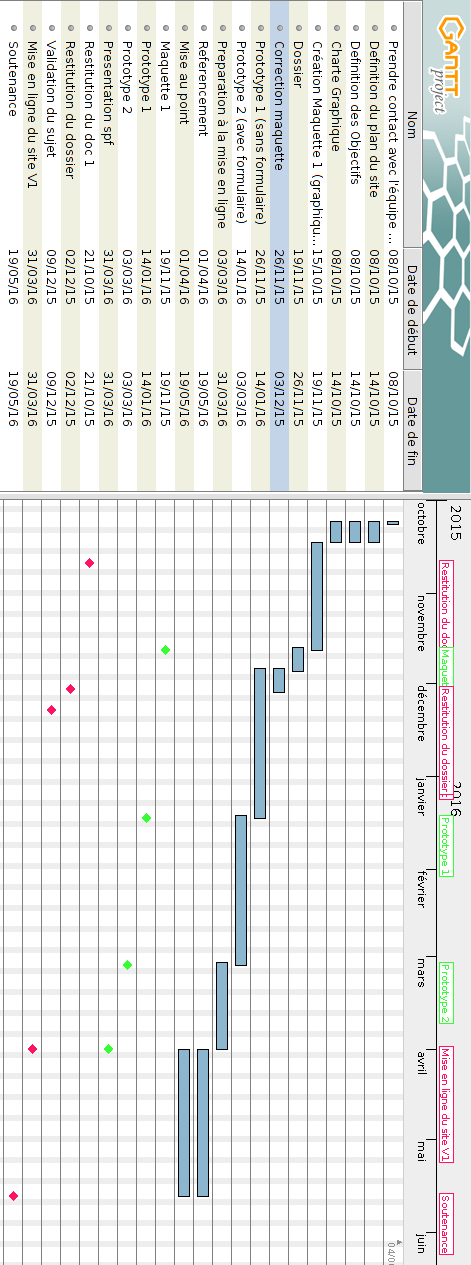
\includegraphics[width=16cm]{gantt.png}
\newpage
\section{Première Réunion - 8/10/15}
La première réunion en présence de Mr Redou nous a permis de prendre conscience de l'envergure du travail a fournir. Nous avons alors constaté qu'il était nécessaire de créer complètement le site. Après discutions nous avons décidé de concentrer notre projet uniquement autour de la création du site dans le but d’être certain de pouvoir fournir le meilleur outil possible.
\section{Seconde Réunion - 15/10/15}
Notre seconde réunion en présence d'une partie de l'équipe d'EntrEmploi nous a permis de nous présenter de mettre a plat le besoin auquel nous pouvons tenter de répondre avec nos ressources. Nous nous sommes mis d'accord sur les objectifs et fonctionnalités à fournir suivantes:\\
Objectifs:
\begin{itemize}
    \item Faire connaître Entr'Emploi
    \item Donner envie à des chercheurs d'emploi de faire appel a Entr'Emploi
    \item Donner envie aux recruteurs d'utiliser le site
    \item Faire connaître la fédération
\end{itemize}
Fonctionnalités:
\begin{itemize}
    \item Présentation du projet
    \item Prestation
    \item CVthèque
    \item Offres d'emploi
    \item Liste de partenaires
    \item Lien vers la fédération/don/bénévolat
\end{itemize}
Nous avons également choisi de reprendre le code couleur du logo du secours populaire pour la charte graphique en nous basant également sur le site du secours populaire.
\section{Troisième Réunion - 19/11/15}
En présence d'une plus grande partie de l'équipe nous avons présenté une maquette du site dans le but de clarifier les attentes de l'équipe envers le site. Nous avons également rencontré le bénévole qui sera responsable de la mise à jour du contenu du site.\\
Nous avons également discuté de la présence des différents logos et de l'importance que le site soit clairement en lien avec le secours populaire, en particulier la présence de redirections vers les pages de dons et de bénévolat du secours populaire.\\
Pour finir, après avoir écouté différentes suggestions et inquiétude de l'équipe nous nous sommes mis d'accord sur une liste de changement à effectuer sur la maquette et sur notre planning qui prévoit une autre réunion en janvier.\\
Une réflexion sur le nom de domaine doit encore être faite autour de ses différents noms de domaines:
\begin{itemize}
    \item www.entremploi.org
    \item www.entremploi29.org
    \item www.entremploi26.bzh (coût élevé)
    \item www.entremploi.secourspopulaire.fr
    \item www.entremploi.spf29.org
\end{itemize}
\end{document}
